	\chapter{Convolutional Neural Networks}
	\section{CNNs Frequently Asked Questions}

	\resetquestioncounter{}
	\begin{qanda}
		\begin{question}
 What is Computer Vision?
		\end{question}
		\begin{answer}
Computer Vision is a field of Artificial Intelligence that enables computers or systems to derive or extract meaningful information from a digital image or video data and take actions or recommendations based on this information.
		\end{answer}
	\end{qanda}

	\begin{qanda}
		\begin{question}
 What is the Normalization of pixels?
		\end{question}
		\begin{answer}
For most image data, the pixel values are integers with values between 0 and 255. Normalization scales these pixel values between 0 and 1 before modeling.
		\end{answer}
	\end{qanda}

	\begin{qanda}
		\begin{question}
Why should Normalization be performed on pixels?
		\end{question}
		\begin{answer}
Neural networks process inputs using small weight values and inputs with large integer values can disrupt or slow down the learning process, so it is a good practice to normalize the pixels so that the values would range between 0 and 1.
		\end{answer}
	\end{qanda}

	\begin{qanda}
		\begin{question}
How is smoothing performed on images?
		\end{question}
		\begin{answer}
Smoothing an image is required to reduce noise and blur the false edges. Smoothing is usually performed using Gaussian Blur. Gaussian filtering is highly effective at removing noise from the image. We can use the below code to perform Gaussian Blur.

		\begin{code}[\codenumbering]{}
			\codeitemnonumber blur\_image = cv2.GaussianBlur(original\_image, (5,5), 0)
		\end{code}
		\end{answer}
	\end{qanda}

	\begin{qanda}
		\begin{question}
Will the images always be provided in zip file format?
		\end{question}
		\begin{answer}
The image data sets are usually provided in the following formats:

	\begin{bulletedlist}
		\item {\bfseries Folders/Directories}: The whole data set can be given in a single directory or a zip file which can be extracted to get a directory. This directory can contain sub-folders like training and testing. The training and testing folders may contain individual sub-folders for each category of image. The whole structure can be observed in the \figurename~\ref{fig:cnnimagesinfiles}.
		\item {\bfseries TensorFlow data sets}: The data sets can be loaded from as shown in \figurename~\ref{fig:cnntensorflowdataset}.
		\item {\bfseries numpy arrays}: The images can also be given as numpy arrays and the labels to the corresponding images can be given in a CSV file.  The images that are converted into numpy arrays can be given in \textcode{images.npy} file and the labels corresponding to each image can be given in the \textcode{labels.csv file}.  The \textcode{np.load()} function can be used to read the numpy arrays and the \textcode{pd.read\_csv()} function from pandas can be used to read the \textcode{csv} file as shown in \figurename~\ref{fig:cnnnumpyarraydataset}.
	\end{bulletedlist}
		\end{answer}
	\end{qanda}

	\begin{figure}[h]
		\centering
		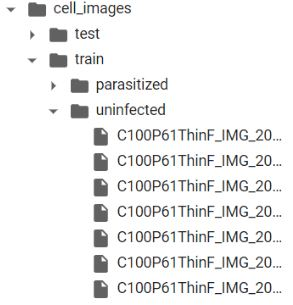
\includegraphics[height=2in]{cnnimagesinfiles}
		\caption[Cross validation]{Cross validation.}
		\label{fig:cnnimagesinfiles}
	\end{figure}

	\begin{figure}[h]
		\centering
		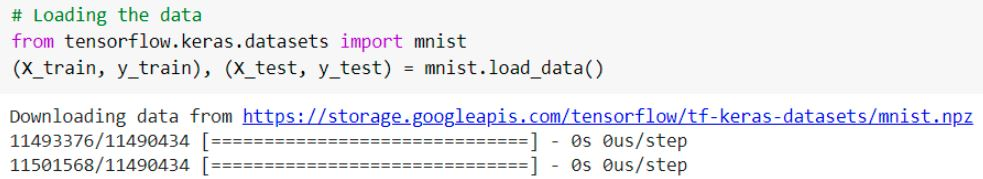
\includegraphics[width=\textwidth-1in]{cnntensorflowdataset}
		\caption[Loading a TensorFlow image data set]{Loading a TensorFlow image data set.}
		\label{fig:cnntensorflowdataset}
	\end{figure}

	\begin{figure}[h]
		\centering
		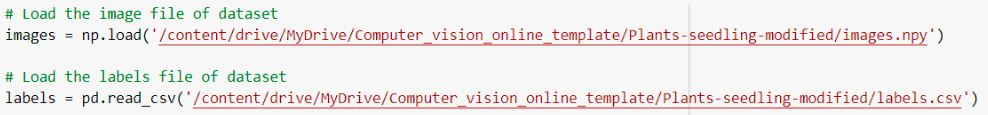
\includegraphics[width=\textwidth]{cnnnumpyarraydataset}
		\caption[Numpy array loading of image data set]{Numpy array loading of image data set.}
		\label{fig:cnnnumpyarraydataset}
	\end{figure}

	\begin{qanda}
		\begin{question}
Do we need to split the image data into train and test sets before pre-processing?
		\end{question}
		\begin{answer}
The splitting of image data should be performed before any operations or pre-processing steps on images.  One way is to divide the data set into two subsets:
	\begin{numberedlist}
		\item Training set: a subset to train a model.
		\item Test set: a subset to test the model.
	\end{numberedlist}

Separating the data enables you to evaluate your model generalization capabilities and have an idea of how it would perform on unseen data.  Good performance on the test set is a useful indicator of good performance on new data in general, assuming that:
	\begin{bulletedlist}
		\item The samples were drawn independently and at random from the distribution to create the test set.
		\item The test set is large enough.	
	\end{bulletedlist}

The second way is to divide the data set into three subsets:
	\begin{numberedlist}
		\item Training set: a subset to train a model.
		\item Validation set: a subset to validate and tune our model.
		\item Test set: a subset to test the model.
	\end{numberedlist}
		\end{answer}
	\end{qanda}

	\begin{qanda}
		\begin{question}
What is the difference between MNIST and Fashion MNIST data sets that are used in the course?
		\end{question}
		\begin{answer}
The MNIST data consists of images of 10 handwritten digits from 0 to 9, and this data set can be directly loaded using the \textcode{load\_data()} function of TensorFlow.  Whereas, Fashion MNIST can also be loaded using the same \textcode{load\_data()} function, it consists of fashion images like shoes, shirts, etc belonging to 10 different categories.
		\end{answer}
	\end{qanda}

	\begin{qanda}
		\begin{question}
What is the difference between \textcode{resize()} and \textcode{reshape()} functions (in context of images)?
		\end{question}
		\begin{answer}
The \textcode{reshape()} function changes the shape only and not the number of pixels.  For example, the image of size 6 x 4 can be reshaped into 12 x 2.  Here we did not change the number of pixels.  But an image of 6 x 6 can be resized into 10 x 10 using the resize function.  Here the number of pixels are increased.
		\end{answer}
	\end{qanda}

	\begin{qanda}
		\begin{question}
Which function can be used to get the names of labels that are encoded using an encoder?
		\end{question}
		\begin{answer}
The \textcode{inverse\_transform()} function can be used to decode the labels from the encoded vectors.  For example: if a label ``car'' is encoded using a label binarizer into an array of [0,0,1] then \textcode{inverse\_transform()} can be used to get the label name from this array.
		\end{answer}
	\end{qanda}

	\begin{qanda}
		\begin{question}
How to unzip a zipfile in Google Colab?
		\end{question}
		\begin{answer}
The unzip command can be used to unzip the file in Google Colab.
		\begin{code}[\codenumbering]{}
			\codeitemnonumber !unzip ``path to the file''
		\end{code}
		\end{answer}
	\end{qanda}


	\section{ANNs versus CNNs}
	\subsection{Image Classification Using ANNs}
	\subsubsection{Method}

	\begin{bulletedlist}
		\item If the images are RGB, we know that each image will have 3 channels, which will be represented by 3 matrices - each matrix numerically representing the pixel intensity values from that channel.
		\item The information about brightness, contrast, edges, shape, texture, shadows etc. of an image does not depend on color. So the RGB representation of images only adds to the complexity, and may be replaced by their gray scale version instead.
		\item For that reason, we will use the gray scale color space, which isolates the color information into a single channel.
		\item In ANNs, one neuron would be used for each input (\figurename~\ref{fig:imageprocessingwithann}). Here the inputs are the pixel values in an image.  For an image with 28 x 28 pixels, the flattened input layer will have 28*28 = 784 inputs.
		\item Every node/element in the output vector refers to an output class.  The input sample is labeled according to the class with the highest score.
	\end{bulletedlist}

	\begin{figure}[tbh]
		\centering
		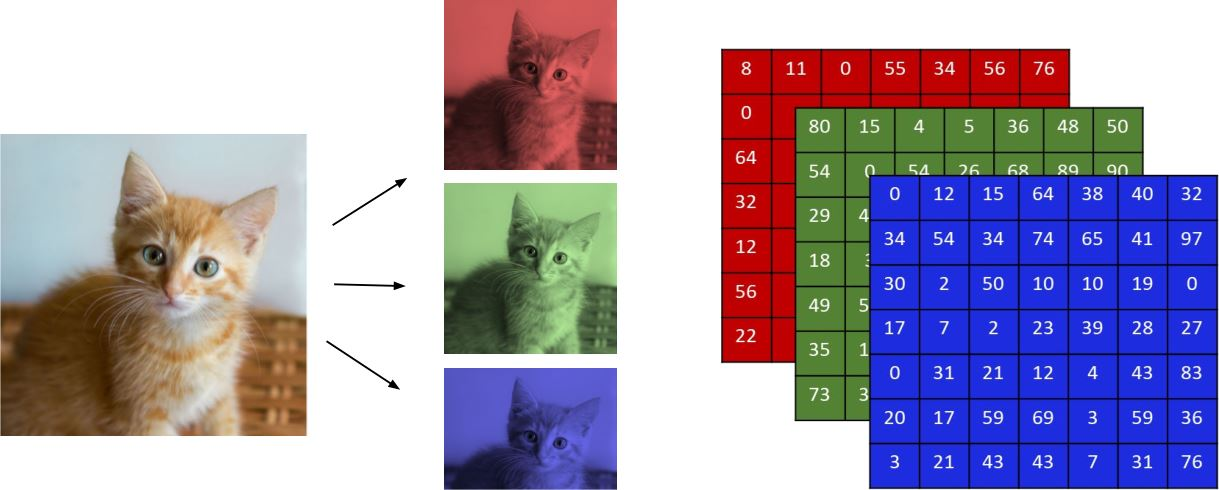
\includegraphics[height=1.5in]{catimagetorgbchannels}
		\caption[Image broken down into RGB channels]{Image broken down into RGB channels.}
		\label{fig:catimagetorgbchannels}
	\end{figure}

	\begin{figure}[tbh]
		\centering
		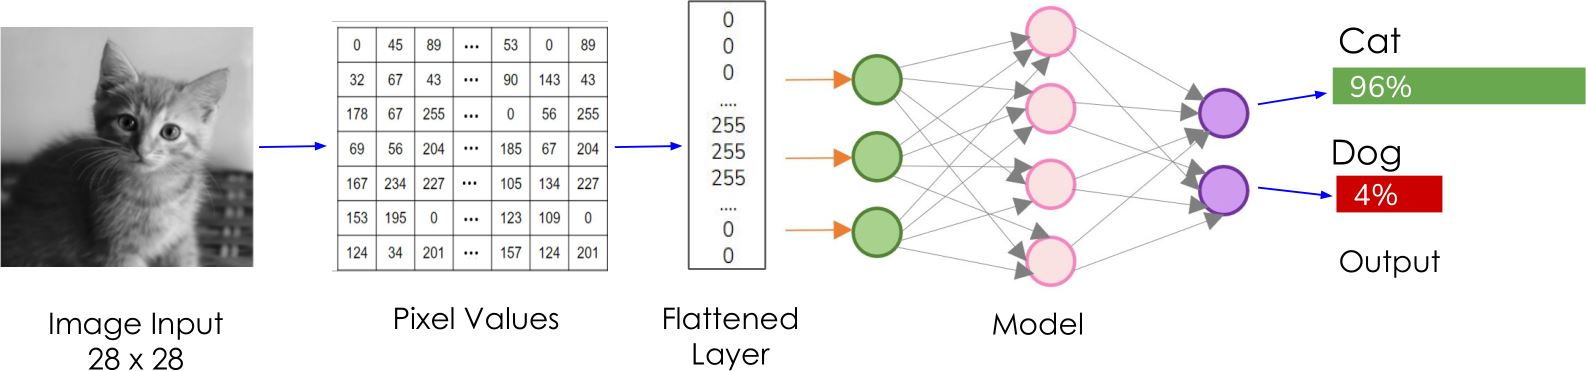
\includegraphics[width=\textwidth]{imageprocessingwithann}
		\caption[Image processing with ANNs]{Image processing with ANNs.}
		\label{fig:imageprocessingwithann}
	\end{figure}


	\subsubsection{Challenges with Image Classification Using ANNs}

	\begin{bulletedlist}
		\item One of the main disadvantages of ANNs is that \textbf{they are not translation invariant}.  For example, a cat may be present in the center, left, or right of an image.  ANNs would try to learn the location the cat is present as an indicator of its presence.  This may give inconsistent results.
		\item Another problem with ANNs is that \textbf{they lose spatial information} after getting the image matrix converted into a flattened array.  This means ANNs do not leverage the fact that nearby pixels are more strongly related than distant ones.
		\item Yet another disadvantage of ANNs for image classification, has to do with detecting which features of an image are important and which ones are not. When detecting the presence of the object, there is no use of looking at the background or other features of an image. There is unfortunately no scope to use this idea in a traditional ANN, which may give importance to every pixel in an
image, and will hence try to learn the background of the object as well.  For example, a cat remains a cat whether it is in the garden or on a table.  However, an ANN will wrongly learn about the background and assume that a cat appears in a specific background.
	\end{bulletedlist}


	\subsubsection{The Computationally Expensive Nature of ANNs}
	\begin{bulletedlist}
		\item ANNs are very computationally expensive.
		\item To use an ANN, we would first have to flatten the input. Using just two fully-connected layers (of 32 and 2 nodes each) on the input image of 28x28x1, we observe that there are already about 50,000 trainable parameters, and this would just increase with an increase in the number of layers.
	\end{bulletedlist}

	\begin{figure}[tbh]
		\centering
		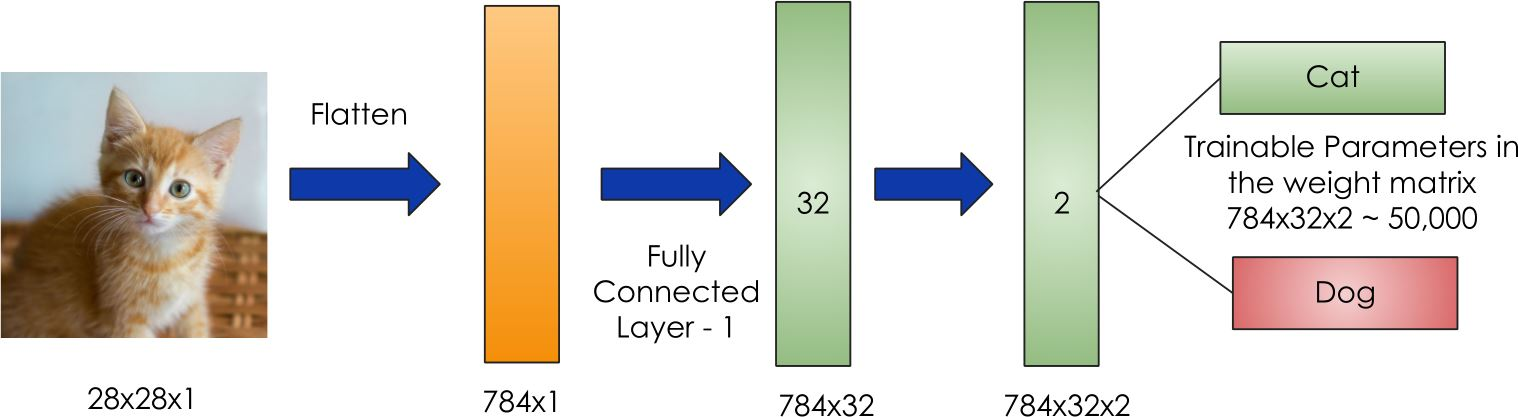
\includegraphics[width=\textwidth-1in]{fullyconnectannforimageprocessing}
		\caption[Expense of image processing with ANNs]{Expense of image processing with ANNs.}
		\label{fig:fullyconnectannforimageprocessing}
	\end{figure}


	\subsection{Spatial and Translational Invariance of CNNs}

	\begin{bulletedlist}
		\item CNNs have the in built property of handling positional shifts, or translations of a given image. They are
spatially and translationally invariant (see \figurename~\ref{fig:translationalinvarianceforcnns}).
		\item In the below example, we have three images of a cat.  It obviously remains a cat regardless of whether it appears in the left, the center or the top right corner of the image.  Unlike ANNs, CNNs are able to understand this, as you would expect for any practical computer vision model.
		\item CNNs achieve this through the use of convolutional and pooling layers.
		\item Convolutional layers extract the right set of features from the image by applying filters that match those patterns in the image. Since the same filter is applied through a sliding mechanism throughout the whole image, the features of the image get detected irrespective of their position.
		\item The result of the convolutional layer is sent to the pooling layer. The pooling layer reduces the image complexity and size, and extracts the important features from the pooling patch. This achieves the dual task of eliminating unwanted background features, as well as the translational invariance of removing the information about the exact position of the object in the image.
		\item This is why CNNs will likely work well even for shifted objects in images, even if the CNN is not explicitly trained on images with such variability.
		\item Each layer in the CNN introduces some amount of translational invariance, and the more layers we add, the more effective it usually becomes.
		\item \textbf{CNNs automatically detect or learn the important features of an image without any human supervision.} For example, in an image data set of handwritten digits, CNNs learn the distinctive features for each digit by themselves, by learning the best filter values through backpropagation.
		\item Convolutional filters change the input in such a way that only the important features are extracted.  In \figurename~\ref{fig:cnnsignorebackground}, detecting the presence of the dog does not require extracting information about the background (depicted in red lines).  We only need to extract the relevant features of the dog, and ignore all other information.  This is achieved using convolution and pooling.
	\end{bulletedlist}

	\begin{figure}[tbh]
		\centering
		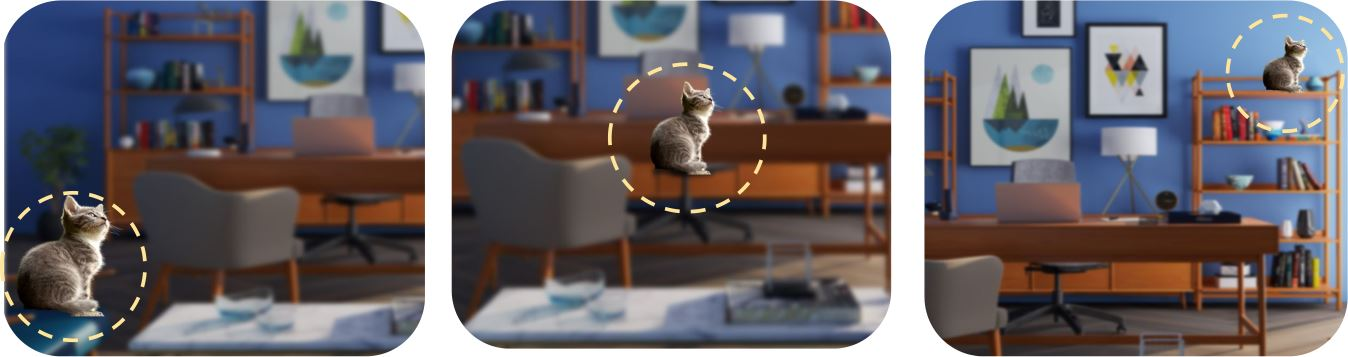
\includegraphics[width=\textwidth-1in]{translationalinvarianceforcnns}
		\caption[Translational invariance for CNNs]{Translational invariance for CNNs.}
		\label{fig:translationalinvarianceforcnns}
	\end{figure}

	\begin{figure}[tbh]
		\centering
		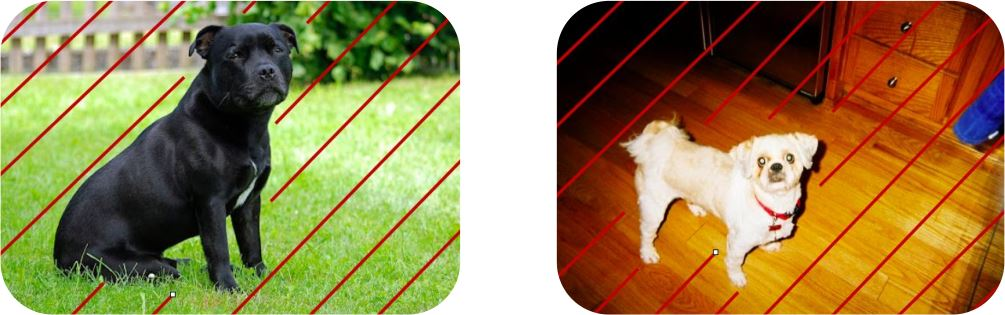
\includegraphics[width=\textwidth-1in]{cnnsignorebackground}
		\caption[CNNs ignore background]{CNNs ignore background.}
		\label{fig:cnnsignorebackground}
	\end{figure}


	\subsection{Computational Advantage of CNNs}
	\begin{bulletedlist}
		\item \textbf{Weight sharing}: In the convolution process, we apply the same filter to every patch of the image.
As a result:
		\begin{bulletedlist}
			\item It reduces the number of weights that must be learned, which reduces training time and cost.
			\item It makes the filter search insensitive to the location of the important features in the image.
		\end{bulletedlist}
		\item Let's say we have an image of size 50x50x3 (i.e.\ 7500 pixels or features) as represented in \figurename~\ref{fig:cnnfeatures}.
		\begin{bulletedlist}
			\item Taking a CNN Layer with 10 filters and a kernel size of 3x3, we'll have the given output of size 48x48x10 size having 23040 features.
			\item Unlike in ANNs, the number of trainable parameters still remains a small fraction of the features and does not scale with that large number.
			\item Number of trainable parameters = (filter size x number of channels + bias) x No. of filters = (3x3x3 + 1) x 10 = 280
		\end{bulletedlist}
	\end{bulletedlist}

	\begin{figure}[tbh]
		\centering
		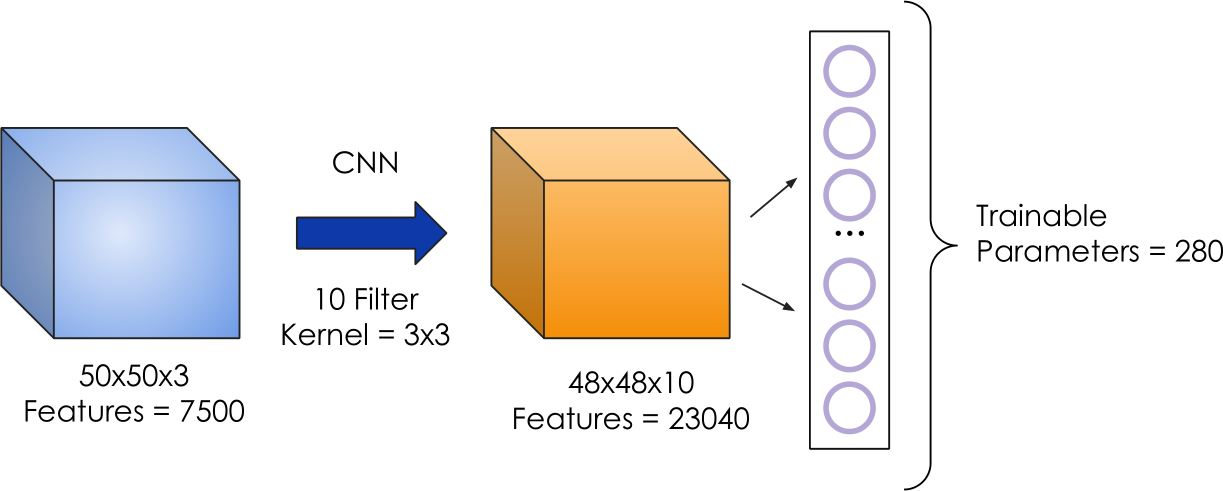
\includegraphics[width=\textwidth-2in]{cnnfeatures}
		\caption[CNNs features]{CNNs features.}
		\label{fig:cnnfeatures}
	\end{figure}


	\subsection{Summary}
	\begin{bulletedlist}
		\item CNNs perform better than ANNs in the crucial task of capturing the relevant features from an image, by ignoring any spatial and translational transformations.
		\item The use of filters in a CNN helps us reduce the dimensionality of the image and extract only the important and required information.
		\item Convolutional filters require exponentially less trainable parameters in comparison to the fully-connected dense layers required in ANNs, and this gives CNNs a computational advantage over ANNs as well.
	\end{bulletedlist}

	\section{CNN Architecture}
	\begin{bulletedlist}
		\item The CNN architecture for image classification is comprised of two major parts:
		\begin{numberedlist}
			\item The feature extraction stage with (a) Convolution layer + Activation function and (b) Pooling layer.
			\item The prediction stage with (a) Flatten layer and (b) Fully connected layer.
		\end{numberedlist}
	\end{bulletedlist}

	\begin{figure}[tbh]
		\centering
		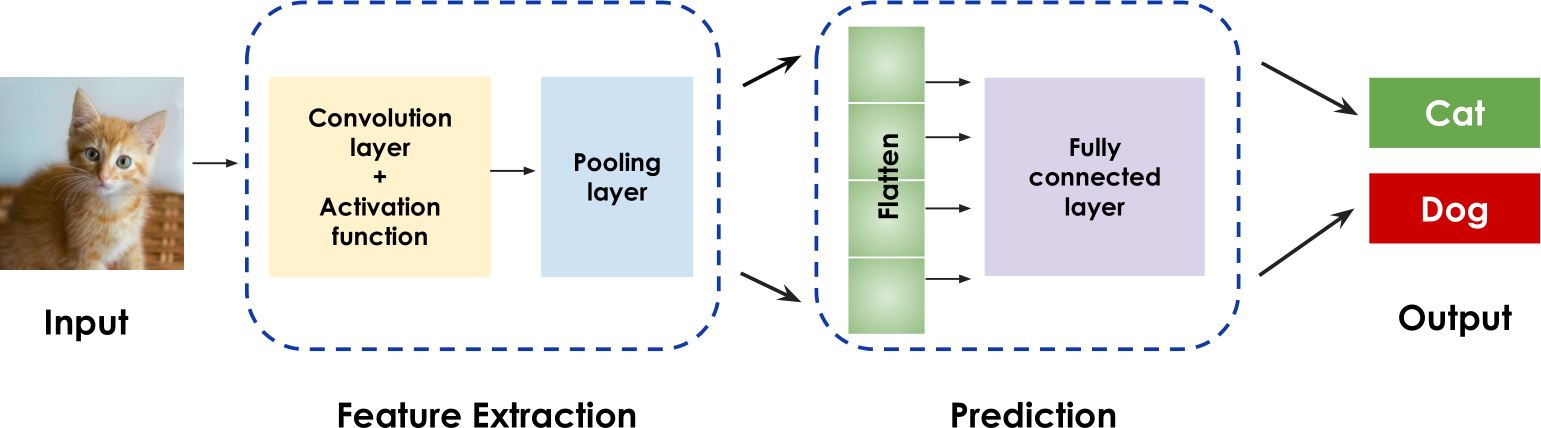
\includegraphics[width=\textwidth-1in]{cnnarchitecture}
		\caption[CNNs architecture]{CNNs architecture.}
		\label{fig:cnnarchitecture}
	\end{figure}


	\subsection{Convolutional Layer}
	\begin{bulletedlist}
		\item In the convolutional layer, a filter is applied on an input image to build a feature map.
		\item Filters can be custom made.  In convolutional neural networks though, the values of the filters are learned through training to determine the important features that can categorize the image more accurately. We simply pass the number of filters and their sizes to the CNN, and the model learns the filter values to develop various feature maps that capture the presence of the features detected.
	\end{bulletedlist}

	\begin{figure}[tbh]
		\centering
		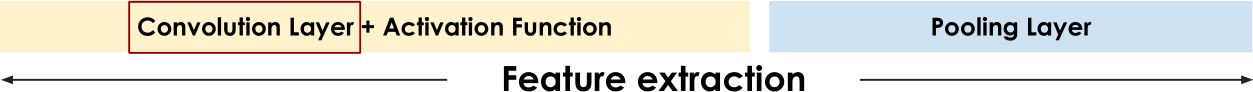
\includegraphics[width=\textwidth-1in]{cnnfeatureextraction}
		\caption[CNN feature extraction]{CNN feature extraction.}
		\label{fig:cnnfeatureextraction}
	\end{figure}

	\begin{figure}[tbh]
		\centering
		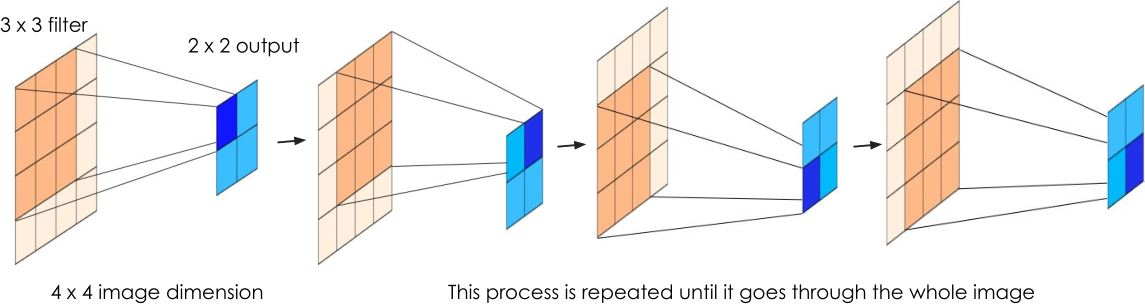
\includegraphics[width=\textwidth-1in]{cnnconvolution}
		\caption[CNN convolution]{CNN convolution.}
		\label{fig:cnnconvolution}
	\end{figure}


	\subsubsection{Activation Function}
	\begin{bulletedlist}
		\item The next step is the Activation Function. In CNNs, the ReLU activation function is used to incorporate a non-linear component into neural networks.
		\item The ReLU function is used in CNNs because the convolution operation is essentially a linear operation (a sum of element-wise products) between the image and the filter, and ReLU adds the non-linearity required for this operation to be able to detect complex non-linear boundaries in the image.
		\item One advantage of using ReLU (Rectified Linear Unit) is that if there are any negative pixels, the function will convert it into zero. This is useful for visualizing these image maps, since negative pixels have no meaning, and it makes subsequent computations more efficient since zeros are easy to work with.
	\end{bulletedlist}

	\begin{figure}[tbh]
		\centering
		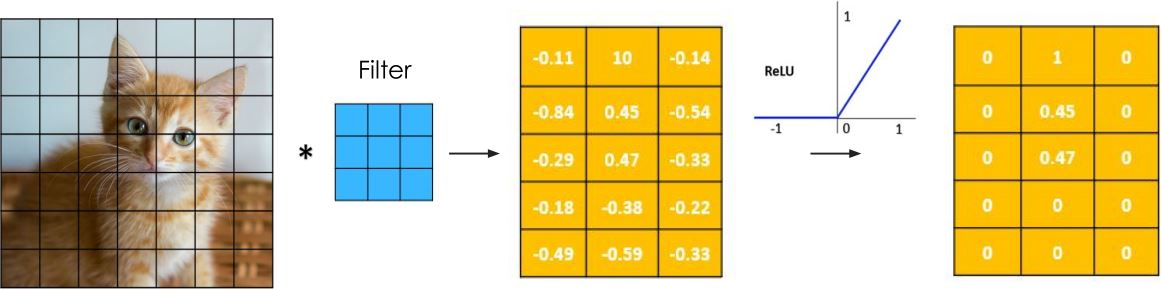
\includegraphics[width=\textwidth-1in]{cnnactivationfunction}
		\caption[CNN activation function]{CNN activation function.}
		\label{fig:cnnactivationfunction}
	\end{figure}


	\subsubsection{Pooling Layer}
	\begin{bulletedlist}
		\item The next step in the Feature Extraction stage is Pooling.  The pooling layer helps in removing unwanted features from the image.  In doing so, it reduces the size of the image and hence decreases the computational cost of the model.
		\item CNNs can use `Max Pooling' (see \figurename~\ref{fig:maxpooling}) to create a pooled feature map using only the maximum values of each patch, and dispose of the unnecessary pixel information.
		\item An important question here is - Do we lose information in this process?  The answer is Yes.  The final feature map includes fewer cells and thus less information than the original input image.  But, the purpose of this step is to discard irrelevant features so that the network can do its job more efficiently.
		\item This process is what's responsible for the ``spatial invariance'' property of CNNs.  Pooling also reduces the size of the images, and hence the number of parameters, which minimizes the likelihood of ``over fitting'', which neural networks are often susceptible to.
	\end{bulletedlist}


	\subsubsection{Flatten Layer}
	\begin{bulletedlist}
		\item After the Feature Extraction stage, we move to the Prediction stage of the CNN.  The first step of the Prediction stage is the Flatten layer.
		\item In this layer, the CNN literally flattens the pooled feature map into a column vector, and the output is used in a standard artificial neural network configuration, which are the fully connected layers of the CNN.
	\end{bulletedlist}

	\begin{figure}[tbh]
		\centering
		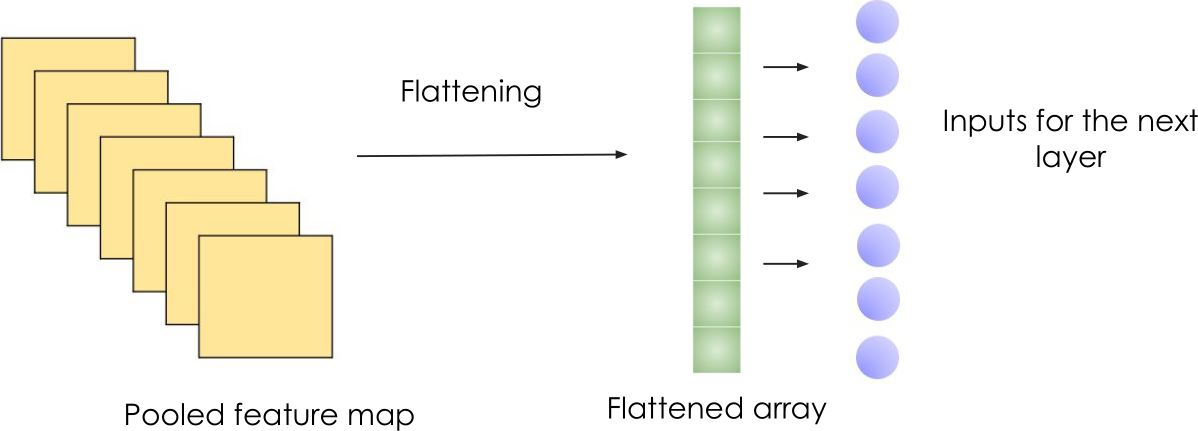
\includegraphics[width=\textwidth-2.0in]{cnnflattenpooledfeaturemap}
		\caption[Flattening pooled features maps to an array]{Flattening pooled features maps to an array.}
		\label{fig:cnnflattenpooledfeaturemap}
	\end{figure}


	\subsubsection{Fully Connected Layer}
	\begin{bulletedlist}
		\item So far, we have learned about the convolution operation, the activation function, pooling and flattening. The final stage of the process is the fully connected layer, where the information from the previous layers is sent to an artificial neural network architecture with Dense (fully connected) layers.
		\item The aim of this step is to take the input and combine the features into a wider variety of attributes that make the convolutional network more capable of categorizing images, which is the sole purpose of building a convolutional neural network.
	\end{bulletedlist}


	\section{Building a CNN Model}
	\begin{bulletedlist}
		\item Let's say we want to build a simple Convolutional Neural Network (CNN) for a prediction problem.  Let's say we need to classify an image as a dog or a cat.
		\item We can build a simple CNN with convolution and pooling layers to solve this problem.
	\end{bulletedlist}

	\begin{figure}[tbh]
		\centering
		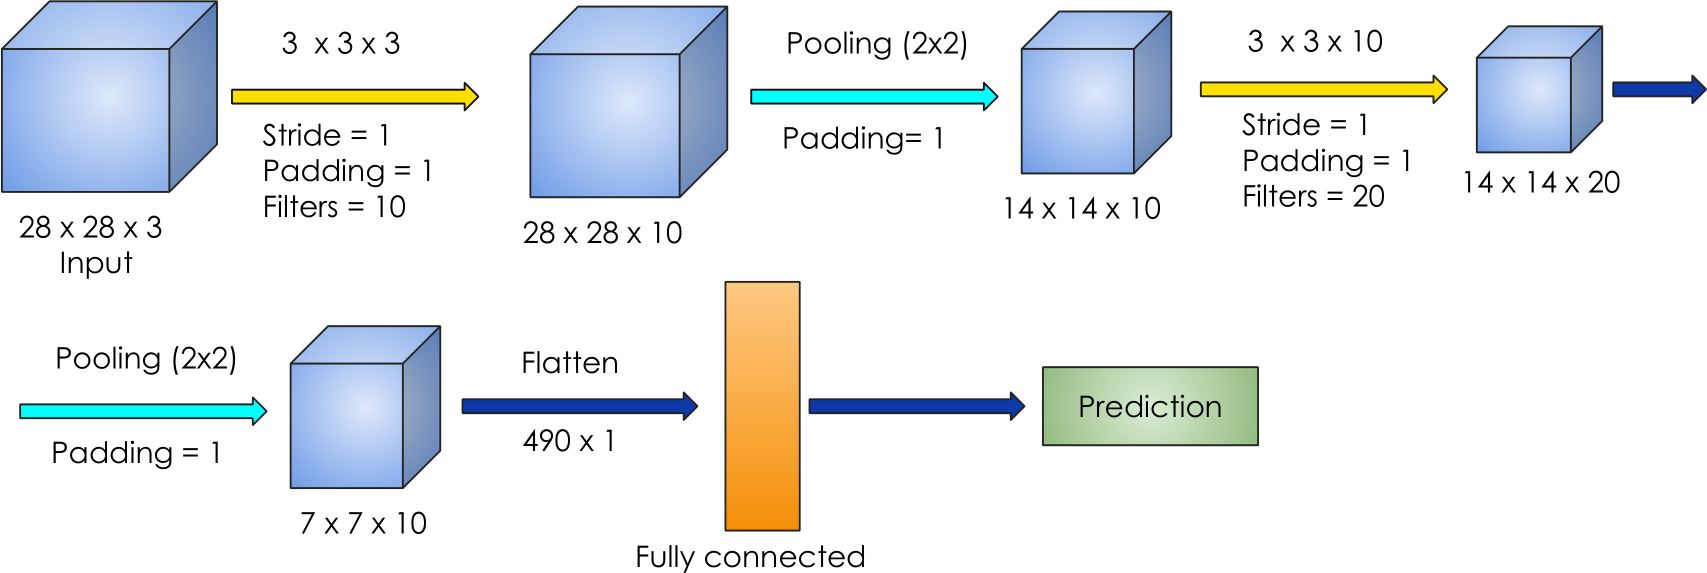
\includegraphics[width=\textwidth-0.75in]{cnnexamplesetup}
		\caption[CNN basic example]{CNN basic example.  The fully connected object is meant to represent one or more hidden layers in a neural network.}
		\label{fig:cnnexamplesetup}
	\end{figure}


	\subsection{Summary}
	\begin{bulletedlist}
		\item We are starting off by applying filters to input images in the form of a convolutional layer.
		\item We break up the linearity of the convolution operation, using the ReLU activation function.
		\item We reduce the image dimension using pooling, for isolating the important features and computational efficiency.
		\item We flatten the feature map and feed it into a fully-connected neural network to generate the final predictions.
		\item Throughout this process, the trainable parameters of the CNN - the weights and filter values, are trained and continuously updated through backpropagation so that the CNN can achieve its best possible performance in image prediction tasks.
	\end{bulletedlist}


	\section{Introduction}
Convolution neural networks are a special type of neural network designed to work with image data.  CNNs use convolutional layers hidden layers which perform convolution operations.  They have some different characteristics to artificial neural networks.
	\begin{bulletedlist}
		\item Unlike ANNs, CNNs capture the spatial structure of the image.
		\item CNNs follow the concept of parameter sharing i.e. one filter is applied over the whole image, because of which they are much more computationally efficient.
		\item The first part in this architecture is the convolutional layer followed by the pooling layer and the second part is the fully connected layer.  This whole architecture is called a convolutional neural network.
	\end{bulletedlist}

	\begin{figure}[h]
		\centering
		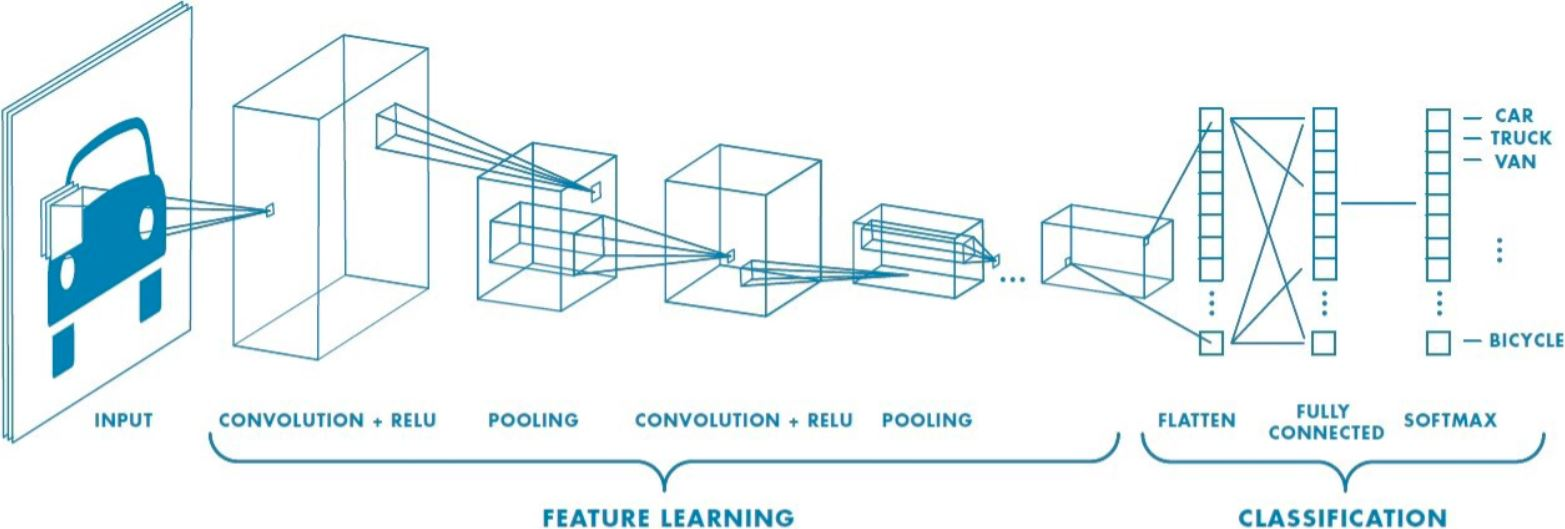
\includegraphics[width=\textwidth-0.5in]{convolutionneuralnetwork}
		\caption[Convolution neural network]{Convolution neural network.  Image source \href{https://towardsdatascience.com/a-comprehensive-guide-to-convolutional-neural-networks-the-eli5-way-3bd2b1164a53}{toward data science}.}
		\label{fig:convolutionneuralnetwork}
	\end{figure}


	\section{Convolutional Layer - Filter/Kernel}
	\begin{bulletedlist}
		\item A convolution operation uses a small array of numbers called a filter/kernel on the input image.
		\item Each filter is designed to identify a specific feature in the input space of the image, such as horizontal edges, vertical edges etc.
		\item A CNN is able to successfully capture the spatial and temporal dependencies in an image through the application of relevant filters.
		\item The role of the CNN is to reduce the images into a form which is easier to process, without losing features which are important for getting a good prediction.
		\item The convolution is performed as shown in \figurename{}s~\ref{fig:convolutionoperationstepsa} and~\ref{fig:convolutionoperationstepsb}.
	\end{bulletedlist}


	\section{Pooling Layer in CNNs}
	\begin{bulletedlist}
		\item After a convolution operation, we usually perform pooling to reduce the dimensions of the feature map.
		\item It enables us to reduce the number of parameters, which both reduces the training time and the over fitting.
		\item Pooling layers down sample each feature map independently, reducing the height and width, but keeping the depth same.
		\item There are two types of pooling - Max and Average.  Max pooling just takes the maximum value whereas average pooling takes the average value in the pooling window (see \figurename~\ref{fig:poolingtypes}).
		\item Contrary to the convolution operation, pooling has no parameters.
	\end{bulletedlist}

	\begin{figure}[h]
		\centering
		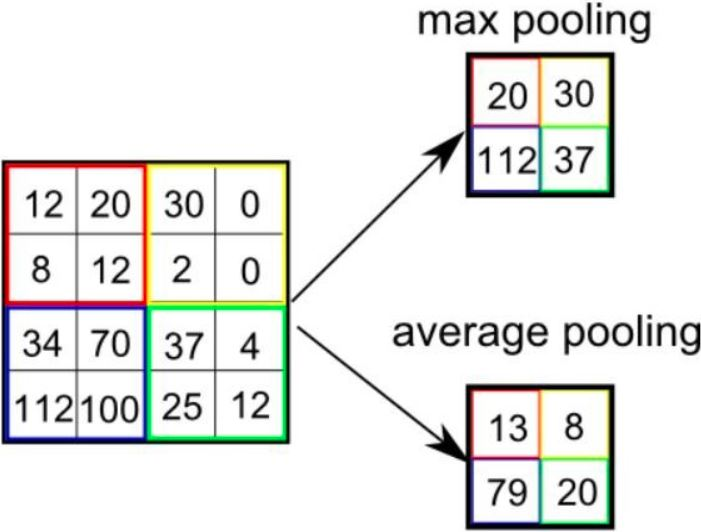
\includegraphics[height=1.5in]{poolingtypes}
		\caption[Types of pooling]{Types of pooling.}
		\label{fig:poolingtypes}
	\end{figure}


	\section{Padding and Stride in CNNs}
	\begin{bulletedlist}
		\item Stride specifies how much we move the filter at each step. By default the value of the stride is 1 and is represented by the first figure
		\item We can also increase the value of stride if we want less overlap between the filters. It also makes the resulting feature map smaller since we are skipping over some locations.
		\item The second figure demonstrates the stride 2.
	\end{bulletedlist}

We see that after using stride, the size of the feature map is smaller than the input. If we want to maintain the same dimensions, we can use padding to surround the input with zeros.  In the following, refer to \figurename~\ref{fig:paddingandstrideincnn}.

	\begin{bulletedlist}
		\item The grey area around the input in the third figure is the padding.
		\item We either pad with zeros or the values on the edge, to match the dimensions of the feature map with the input.
		\item Padding is commonly used in CNNs to preserve the size of the feature maps, otherwise they would shrink at each layer, which is not desirable.
	\end{bulletedlist}

	\begin{figure}[h]
		\centering
		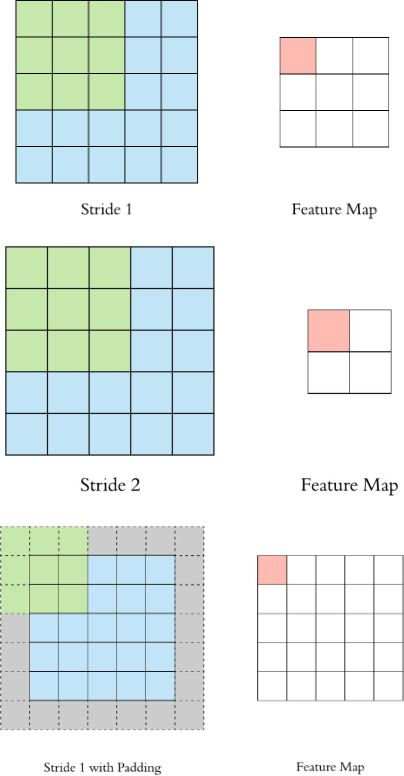
\includegraphics[height=3.5in]{paddingandstrideincnn}
		\caption[Padding and stride in CNNs]{Padding and stride in CNNs.}
		\label{fig:paddingandstrideincnn}
	\end{figure}


	\subsection{Transfer Learning Frequently Asked Questions}
	\begin{qanda}
		\begin{question}
Are there any other Transfer Learning or pre-trained models other than VGG16?
		\end{question}
		\begin{answer}
Yes, there are other pre-trained models like ResNet, EfficientNet, InceptionNet, and MobileNet architectures that can be implemented in TensorFlow.
		\end{answer}
	\end{qanda}

	\begin{qanda}
		\begin{question}
Why should we use Transfer Learning and fine-tune our model?
		\end{question}
		\begin{answer}
The reason is, through experimentation, we observed that early layers of CNN collect basic elements of images such as borders, lines, and so on, whereas subsequent layers capture more specific features such as faces and object shapes. If we use transfer learning, we will need to train the last few layers or the output classifying layer only.

A pre-trained model is trained with data sets that are most likely bigger than your data set. Also, because of reason number 1, and we have trained it with a bigger data set, we have the first few layers that are generalized and hence this helps to reduce over fitting.

Since we are only back propagating within the last few layers, it saves our time and effort.

Architecture-wise, people spend time researching how every feature interacts with an image and hence it is recommended to use this architecture, and published/publicly known result implies that it gives good result.
		\end{answer}
	\end{qanda}

	\begin{qanda}
		\begin{question}
Why should we use GPUs for training the deep learning and the Transfer Learning models?
		\end{question}
		\begin{answer}
GPUs can perform multiple, simultaneous computations. This enables the distribution of training processes and can significantly speed up machine learning operations. With GPUs, we can accumulate many cores that use fewer resources without sacrificing efficiency or power.
		\end{answer}
	\end{qanda}


	\section{Regularization in CNNs}
	\subsection{Over Fitting in CNNs}
	\begin{bulletedlist}
		\item If we only have a limited amount of data to train on, a neural network may be good at recognizing the data that it has been trained. However, it may not perform well on new data, i.e., data it has never seen before (see \figurename~\ref{fig:cnnoverfitting}).
		\item The same is true for Convolutional Neural Networks. They may not be able to perform well on the
test data set, if they have been overtrained on the training data set. There are several
approaches to potentially prevent this over fitting problem.
		\item CNNs can learn filters that fire when a pattern is presented in a given orientation.  However, individual filters in a CNN are not invariant to the rotation of the image.  For example, if we train our model only with images like Image 1 in \figurename~\ref{fig:cnnimagerotation}, the model might think that the pointy ears at the top of the images are a feature of a cat. So, when we test the same model with images like Image 2, which have a rotational component, it will look for pointy ears only at the top of the testing images and not find them, resulting in poor test performance.
		\item This can be avoided if the training data itself includes rotated images.  But finding such data can often be time-consuming and expensive.  That is where Data Augmentation proves its worth.
	\end{bulletedlist}

	\begin{figure}[tbh]
		\centering
		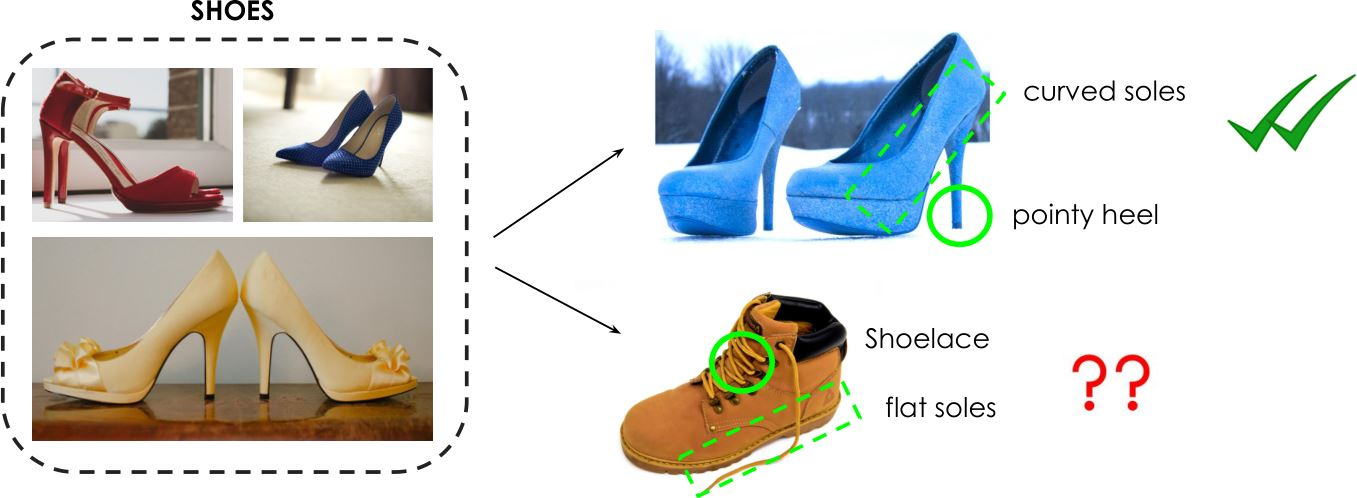
\includegraphics[width=\textwidth-1.5in]{cnnoverfitting1}
		\caption[CNN over fitting]{CNN over fitting.}
		\label{fig:cnnoverfitting1}
	\end{figure}
	\begin{figure}[tbh]
		\centering
		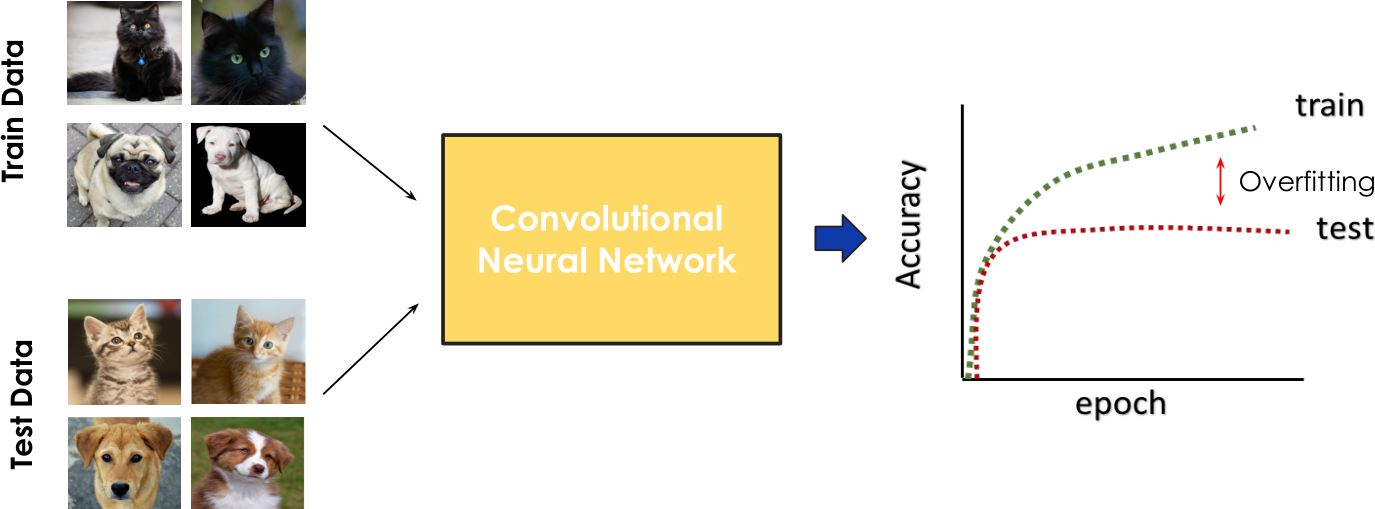
\includegraphics[width=\textwidth-1.1in]{cnnoverfitting2}
		\caption[CNN over fitting]{CNN over fitting.}
		\label{fig:cnnoverfitting2}
	\end{figure}
	\begin{figure}[tbh]
		\centering
		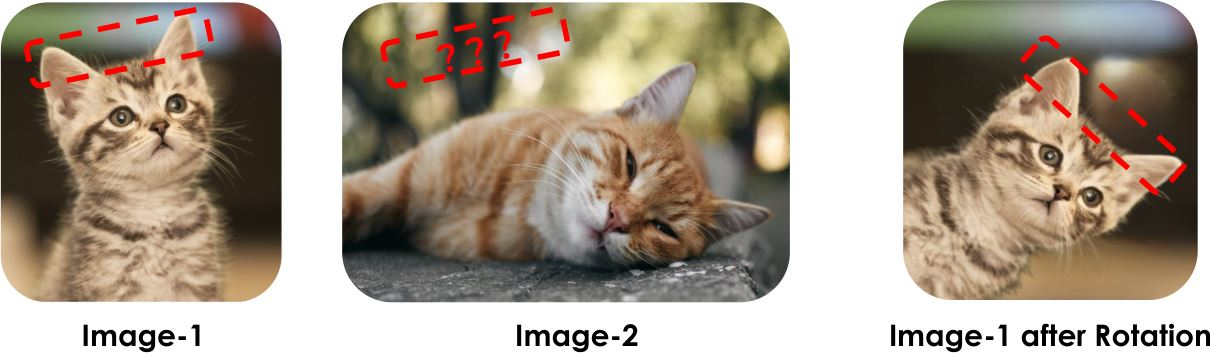
\includegraphics[width=\textwidth-1in]{cnnimagerotation}
		\caption[CNNs and rotation of images]{CNNs and rotation of images.}
		\label{fig:cnnimagerotation}
	\end{figure}

	\subsection{Data Augmentation}
	\begin{bulletedlist}
		\item Data Augmentation is a technique for artificially increasing the size of a training set by generating data from the existing one. Some of the most popular image data augmentation techniques:
		\begin{bulletedlist}
			\item \textbf{Geometric transformations}: Images can be randomly flipped, cropped, rotated, or translated, and that's just the tip of the iceberg.
			\item \textbf{Mixing images}: It is the process of combining different images. Two methods for combining photos are pixel averaging and crop overlaying.
			\item \textbf{Color space transformations}: Changing brightness and contrast, changing RGB color channels, intensify any color.
			\item \textbf{Random erasing}: Deletes a part of the initial image that forces the model to focus on the entire image rather than a portion of it.  This method is inspired by the dropout method that zeros out a random fraction of weights in a neural network layer.
			\item \textbf{Kernel filters}: This technique is used to sharpen or blur images using filters.
		\end{bulletedlist}
		\item The advantage of data augmentation is that all the methods can be used simultaneously, resulting in a large number of distinct data samples from the initial one. We could potentially create millions of images from a single image, due to the exponential growth in the number of combinations possible.
	\end{bulletedlist}

	\begin{figure}[tbh]
		\centering
		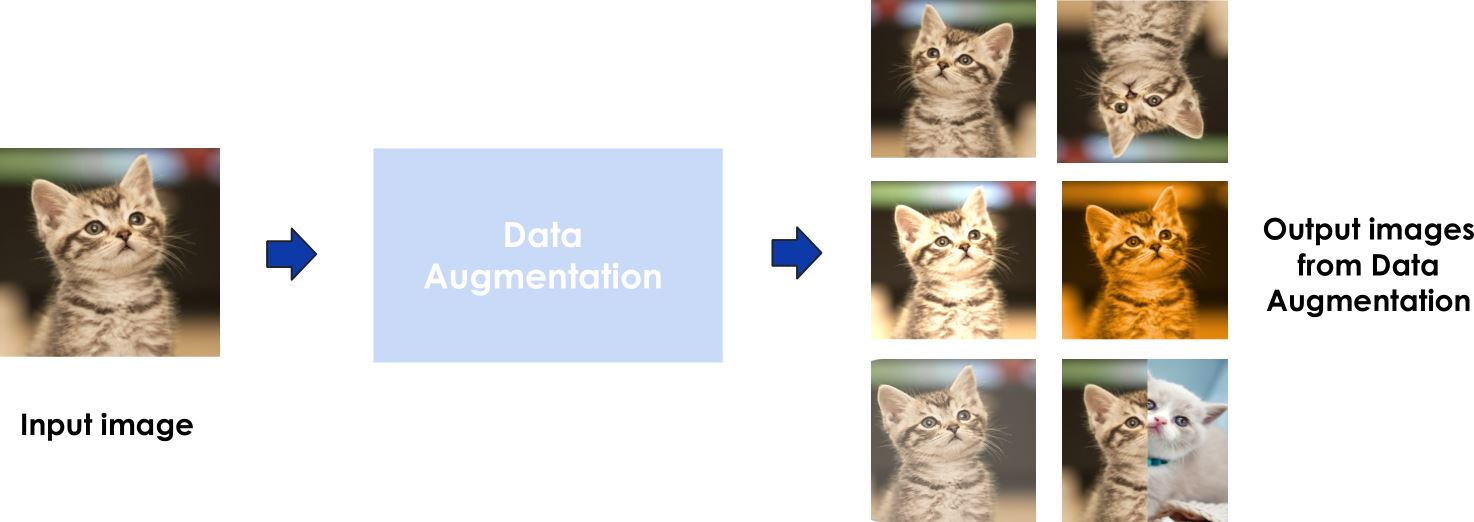
\includegraphics[width=\textwidth-1in]{cnndataaugmentation}
		\caption[Data augmentation for CNNs]{Data augmentation for CNNs.}
		\label{fig:cnndataaugmentation}
	\end{figure}

	\subsection{Batch Normalization}
	\begin{bulletedlist}
		\item Before starting with Batch Normalization, let's discuss why we need normalization and how it helps in speeding up the training process.  The pixel values of an image represent a color code. If we use the images as they are and send them through a Deep Neural Network, the computation of these high numeric values may get costly. Normalizing the values to a range between 0 to 1 will reduce the computational expense.  Consider the example shown in \figurename~\ref{cnnbatchnormalization1}.
		\item Moreover, data points with high values in the non-normalized data set can induce neural network instability. This occurs due to the comparatively large inputs cascading down through the network's layers, which may lead to imbalanced gradients, resulting in the well-known exploding gradient problem.
		\item Normalization reduces variation between the data points by placing all the data on the same scale. This helps prevent exploding gradient problems as there's less variation within data points.  It turns out that scaling data points also makes training a network more efficient and faster.
		\item How is Batch Normalization different from Normalization?  In deep learning, rather than just performing normalization once in the beginning, Batch Normalization is proposed as a technique to scale the output of each layer, specifically by standardizing the activations of each input variable per mini-batch.
		\item Batch Normalization speeds up the training of neural networks by reducing the internal covariate shift.  To better understand covariate shift, consider the following example (shown in \figurename~\ref{fig:covarianceshift}).  Assume that for a cats and dogs classification problem, our model has only been trained on orange cats.  Now, if we were to provide images of white cats while testing, the model may not perform effectively.  This is because of the shift in the input distribution from orange to white, which is known as a covariate shift.
		\item The change in the distribution of inputs to different layers is referred to as the internal covariate shift. While training, each layer tries to fix the error that was introduced during forward propagation. Since every layer is attempting to fix the error that has been created, the update procedure is forever chasing a moving target. More specifically, this process forces the layers to
learn from new input distributions during an update.
		\item Batch Normalization standardizes the activations of each input variable per mini-batch, which means that during the weight update, the assumptions made by the subsequent layer regarding the spread and distribution of inputs will not alter drastically. It turns out that when the distribution of inputs to each layer is similar, training a network is more efficient and faster.
		\item In addition to speeding up learning, Batch Normalization (in short Batch Norm) also provides a weak form of regularization. Since Batch Norm is performed on mini-batches, it adds noise to the data, which results in regularization.
	\end{bulletedlist}

	\begin{figure}[tbh]
		\centering
		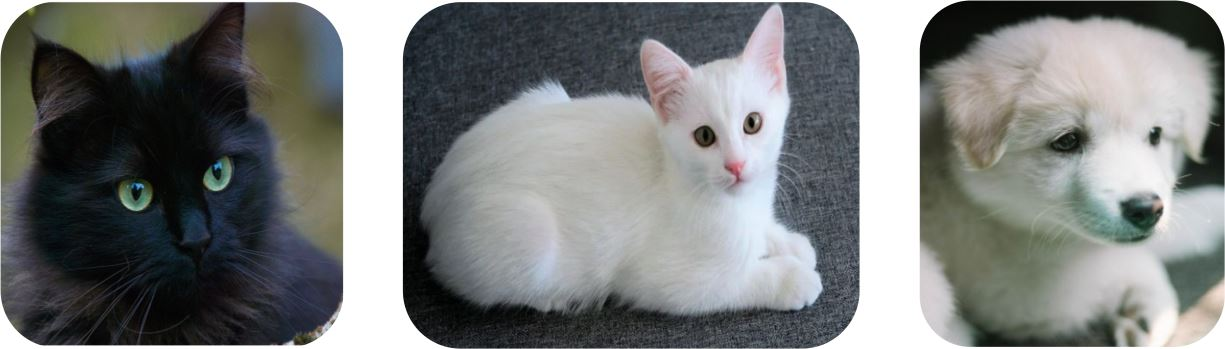
\includegraphics[width=\textwidth-2in]{cnnbatchnormalization1}
		\caption[Example used for batch normalization]{Example used for batch normalization.}
		\label{fig:cnnbatchnormalization1}
	\end{figure}

	\begin{figure}[tbh]
		\centering
		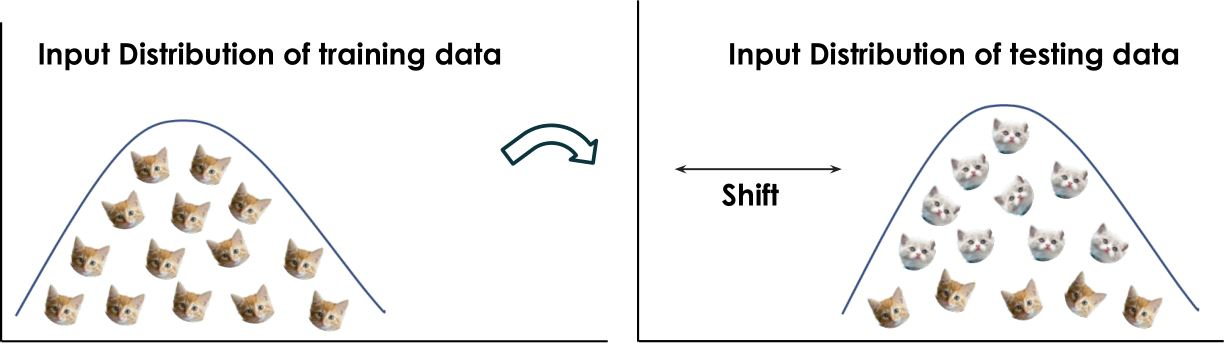
\includegraphics[width=\textwidth-1in]{covarianceshift}
		\caption[Example of covariance shift]{Example of covariance shift.  The input shifted from being from only orange cats to orange and white cats.  This isn't a great example.  Really, it is just any change in the input data.}
		\label{fig:covarianceshift}
	\end{figure}

	\subsection{Spatial Dropout}
	\begin{bulletedlist}
		\item We have already learned about the dropout regularization technique, which is used in neural network training to reduce over fitting.  Let's see how dropout is used after the convolution layer in CNNs.
		\item Convolution between a filter and an input produces feature maps in the convolution layer.  In images, the values of neighboring pixels are highly correlated, resulting in correlated cells in feature maps.  Thus, dropping the cells of feature maps at random using a basic dropout method may not actually prevent over fitting, because even if one cell is removed, the neighboring cell
could give a highly correlated gradient.  That's why we use another idea called Spatial Dropout.
		\item In Spatial Dropout, whole feature maps themselves are randomly dropped.  Dropping a feature map, means making all the cells of that feature map 0, which would be as good as not using it.  Let's suppose we obtained 8 feature maps after the convolution operation. If spatial dropout is applied with dropout probability 0.25, then the expected number of dropped feature maps is 2.
	\end{bulletedlist}

	\begin{figure}[tbh]
		\centering
		\begin{minipage}{\textwidth}
		\centering
		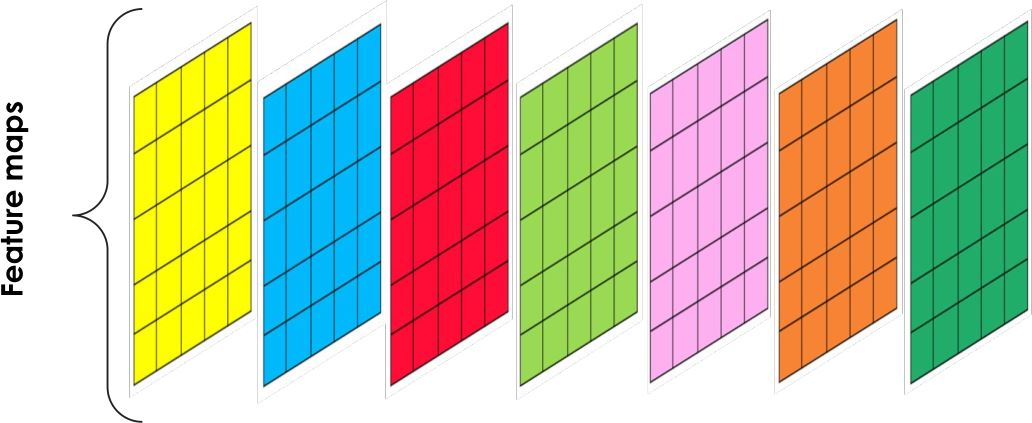
\includegraphics[width=3in]{cnnfeaturemap}
		\end{minipage}
		\begin{minipage}{\textwidth}
		\centering
		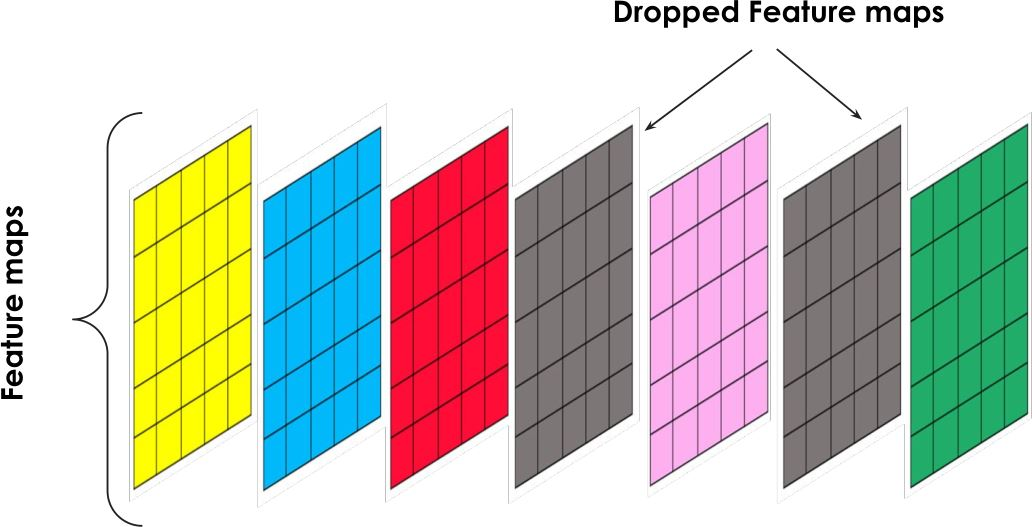
\includegraphics[width=3in]{cnnfeatureextractionwithdropout}
		\end{minipage}
		\caption[Spacial drop out in CNNs]{Spacial drop out in CNNs.}
		\label{fig:covarianceshift}
	\end{figure}

	\section{Introduction to Transfer Learning}
	\subsection{The Ideal CNN model}
	\begin{bulletedlist}
		\item Some of the traits of an ideal and effective Convolutional Neural Network are as follows:
		\begin{bulletedlist}
			\item Low bias
			\item Low variance
			\item High performance metrics (Recall / Precision / F1 Score)
		\end{bulletedlist}
		\item To achieve these measures of success for CNNs, we usually require:
		\begin{bulletedlist}
			\item A large, diverse and high quality labeled image data set,
			\item High computational power to train deep convolutional neural networks for complex images.
		\end{bulletedlist}
		\item However, as we will realize, it is far from straightforward to acquire both the above requirements that are needed to build robust and generalizable Convolutional Neural Networks.
	\end{bulletedlist}

	\subsection{Problems with Training CNNs}
	\begin{bulletedlist}
		\item The first problem has to do with the requirement of a large and diverse labeled image dataset:
		\begin{bulletedlist}
			\item In many domains getting such a large, labeled data set can be very difficult.  Some examples of this:
			\begin{bulletedlist}
				\item Medical Images (X-Rays, CT-Scans, Thermograms, Skin Patch Images)
				\item Agricultural Images (Crop Monitoring, Poultry Farming, Fruit and Vegetable Counting)
				\item Manufacturing Images (Defect Detection, Images of Safety and Security SOPs)
			\end{bulletedlist}
			\item There are challenges with image acquisition such as patient privacy and the prohibitive cost of generating scans using medical equipment in the medical domain, or the labor-intensive, expensive task of acquiring such images in agriculture and  manufacturing.
			\item We also cannot always use Data Augmentation to sidestep the problem of image acquisition, because the training images need to be diverse, meaningful and of high quality.
		\end{bulletedlist}
		\item The second problem is the computational cost of training deep CNNs for state-of-the-art performance with minimal latency.  Even though they are far more computationally efficient than ANNs, training complex and deep CNN models is still a fairly difficult endeavor. It requires Graphical Processing Units (GPUs), Cloud Computing Resources and/or other ideas from accelerated computing hardware. This can be expensive to acquire and may not always be feasible for individual Deep Learning practitioners or algorithmic researchers, who may need to iterate and experiment with model architectures.
	\end{bulletedlist}

	\subsection{Transfer Learning}
	\begin{bulletedlist}
		\item Let's say we have two similar tasks: Task 1 and Task 2
		\item Task 1 has a large, diverse and high-quality labeled training data set, and can be used to train a high-performing CNN. However, let's say we are interested in predictions for Task 2, which perhaps does not have the luxury of such a data set, and only
has a smaller, less diverse labeled data set.
		\item The idea then, is to build a high-performing CNN for Task 1 using the rich data set available for Task 1, and then
transfer that knowledge (the weights, parameters and architecture) to Task 2, such that we don't need to train a model for Task 2 from scratch, and we can use the lower-quality data set for Task 2 just to fine-tune the final model for Task 2.
		\item That is the reason this idea is called ``Transfer Learning.''
		\item The model would initially be trained using the high-quality data set 1 to make predictions for Task 1.
		\item With repeated forward and backward propagations and good hyperparameter selection, we would be able to create an excellent model for Task 1.
		\item This model can then be ``transferred'' to Task 2, and we would then use data set 2 to fine-tune the predictions for Task 2.
		\item The labels/classes of Task 1 and Task 2 will likely be different, so the input and output layers of the model would need to be changed accordingly.  However the bulk of the layers of what could be a deep model would be ``frozen,'' and we could choose to train and adjust the parameters of only the last few layers in the model for Task 2.
		\item Through this, we would be able to build a high-performance model for Task 2, despite not having the data set to do so.
	\end{bulletedlist}

	\begin{figure}[tbh]
		\centering
		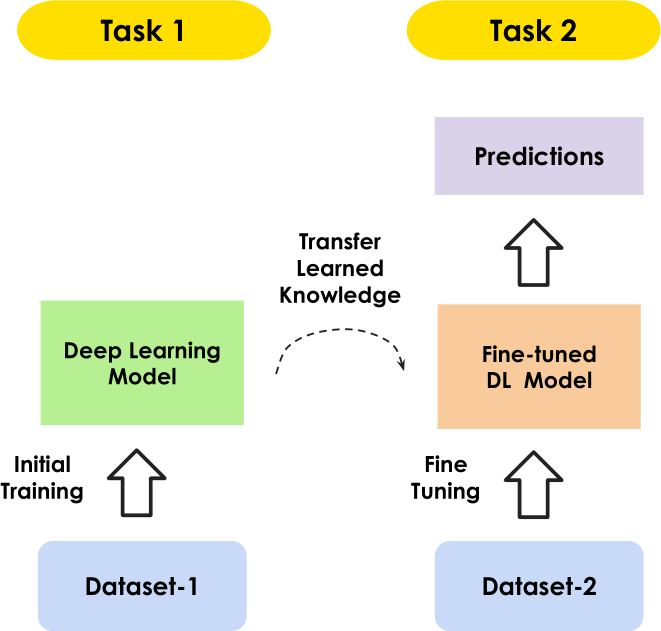
\includegraphics[height=2.5in]{transferlearning}
		\caption[Transfer learning]{Transfer learning.}
		\label{fig:transferlearning}
	\end{figure}

	\subsection{Transfer Learning Terms}
	\begin{bulletedlist}
		\item \textbf{Pre-trained Model}: A model that was previously trained by someone for a particular task, and is
now being transferred and utilized to make predictions for the same task or another task
		\item \textbf{Fine-tuning}: Fine-tuning refers to importing a pre-trained model along with its weights and biases,
and continuing its training with a new data set.
		\begin{bulletedlist}
			\item Here, instead of initializing the weights and biases with random distributions, we initialize them with the weights and biases of the pre-trained model.
		\end{bulletedlist}
		\item \textbf{Transfer Learning}: Transfer Learning is when a pre-trained model is directly used with or without
fine-tuning, to make predictions for another task that is similar to the task that the model was
originally trained on.
		\begin{bulletedlist}
			\item To make such predictions, the feature extraction layer can be ``frozen'' and reused, and only the last prediction layers may be altered according to the labels in the new data set.
		\end{bulletedlist}
	\end{bulletedlist}

	\subsection{Benefits of Transfer Learning}
	\begin{bulletedlist}
		\item At a broader level, Transfer Learning represents a way of reusing the intelligence gained from a high-quality, pre-existing data set to make predictions on new tasks, which may not have data sets of the same quality as the original task the model was trained on. It represents a significant step on the path to a more generalizable form of Artificial Intelligence.
		\item Transfer Learning has been a game-changer in Deep Learning and Artificial Intelligence, because it means individual practitioners can simply ``import'' the latest state-of-the-art Deep Learning architectures from industry giants such as Google and Microsoft and directly utilize them for their own prediction tasks.  The idea is, of course, not just restricted to Computer Vision. It has also been utilized in other areas of AI research, such as Natural Language Processing.
		\item Since these models were trained on huge data sets for a long period of time, it would normally be difficult for other researchers to replicate on their own.  But through Transfer Learning this replication is far easier, and both the earlier problems of CNNs - the lack of access to large, high-quality labeled data sets, and the computational cost of training deep CNN models, can successfully be sidestepped by importing and just fine-tuning these state-of-the-art architectures. The model has already learnt good parameters from a rich data set, and only a few layers of the architecture need to be re-trained and fine-tuned, significantly decreasing the computational cost.
	\end{bulletedlist}


	\subsection{How Transfer Learning work in CNNs}
	\begin{bulletedlist}
		\item As we have learnt in CNNs, the initial convolutional layers of the model extract basic features from the images, and as we go deeper into the architecture, complex features are extracted.
		\item The filters trained initially for extracting the basic features for Task 1, can directly be used for Task 2 to extract similar features, because the understanding of basic features like edges is common to many image processing tasks. This is what helps us prevent the process of training our whole model once again for Task 2 and instead, just transfer the learnings from Task 1 to Task 2.
		\item In Task 2, we only have to fine-tune the last fully-connected layers used for prediction, by utilizing the data set we have for Task 2 to update the weights at the prediction stage.  As only fine-tuning is required, and we don't need to train the model from scratch, this can be done with a small data set and limited computational resources.
	\end{bulletedlist}
	\begin{figure}[tbh]
		\centering
		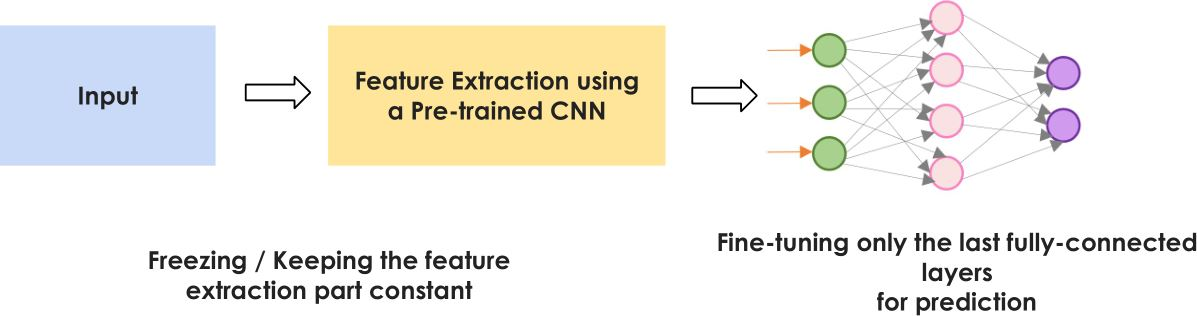
\includegraphics[width=4.5in]{howtransferlearningworks}
		\caption[How transfer learning works]{How transfer learning works.}
		\label{fig:howtransferlearningworks}
	\end{figure}

	\subsection{When to use Transfer Learning}
	\begin{bulletedlist}
		\item Transfer Learning is beneficial in situations where we have:
		\begin{bulletedlist}
			\item A limited amount of labeled training data.
			\item A limited amount of computational power.
		\end{bulletedlist}
		\item However, it is worth keeping in mind the initial premise of Transfer Learning - Task 1 and Task 2 have to be similar.  The level of success of Transfer Learning is correlated with the level of similarity between the two tasks. The more dissimilar the tasks, the more work we have to do on the imported model - instead of simply fine-tuning the last few layers for example, we may also need
to fine-tune some of the latter Convolutional layers or even the whole Convolutional Neural Network, with only the architecture of the network then being reused and not the weights.
	\end{bulletedlist}

	\subsection{Transfer Learning and ImageNet}
	\begin{bulletedlist}
		\item ImageNet is a large, open-source image dataset containing nearly 14 million labeled images, belonging to over 20,000 categories. Each category usually consists of over a hundred images.
		\item Some of the image classes in ImageNet comprise various animals, birds, reptiles, cars, buses, flowers, plants, and many other objects.
		\item Owing to the complexity of this multi-class classification problem, ImageNet has been one of the most important open-source contributors to have advanced the state-of-the-art in Deep Learning methods for Computer Vision. The annual ImageNet competition - ImageNet Large Scale Visual Recognition Challenge (ILSVRC), has been a testing ground for organizations to evaluate and
improve the performance of their state-of-the-art model architectures.
		\item Due to the large volume of diverse, high-quality labeled images on ImageNet, it has functioned as an excellent Task 1 for Transfer Learning models, that can then be imported and fine-tuned into other specialized tasks that may only have smaller, more limited data sets.
		\item Over time, many research organizations, including industry leaders such as Google and Microsoft, have trained deep, complex Convolutional Neural Networks on ImageNet.  The deep models trained on this data set have been imported and have further been used in many other image prediction tasks, by leveraging Transfer Learning.
		\item These models have proven to be highly useful, and have achieved good performance metrics in many other tasks / problem domains where the availability of such large, labeled training data sets is difficult.
		\item Some examples of these famous model architectures are VGG-16/19, InceptionNets and ResNets.
	\end{bulletedlist}

	\begin{figure}[tbh]
		\centering
		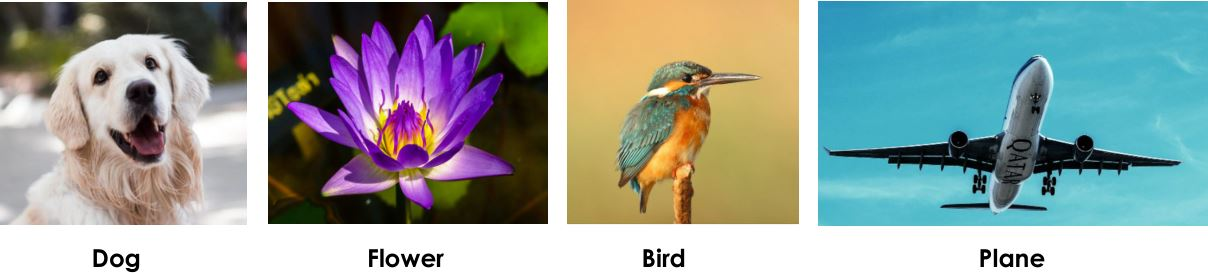
\includegraphics[width=4.5in]{examplesfromimagenet}
		\caption[Examples from ImageNet]{Examples from ImageNet.}
		\label{fig:examplesfromimagenet}
	\end{figure}

	\subsection{Transfer Learning Architectures - VGGNet}

	\begin{bulletedlist}
		\item The VGGNet architecture was proposed by Karen Simonyan and Andrew Zisserman, from the Visual Geometry Group (VGG) at the
University of Oxford, in 2014. It even finished first runner-up in the ImageNet annual competition (ILSVRC) in 2014.
		\item VGGNet has two variants: VGG16 and VGG19. Here, 16 and 19 refer to the total number of convolution and fully connected layers present in each variant of the architecture.
		\item In comparison to previous Deep Learning models for Computer Vision, VGGNet stood out for its simplicity and the standard,
repeatable nature of its blocks. Its main innovation over standard CNNs was simply its increased depth (number of layers) - otherwise
it utilized the same building blocks - convolution and pooling layers, for feature extraction.
	\end{bulletedlist}

	\begin{figure}[tbh]
		\centering
		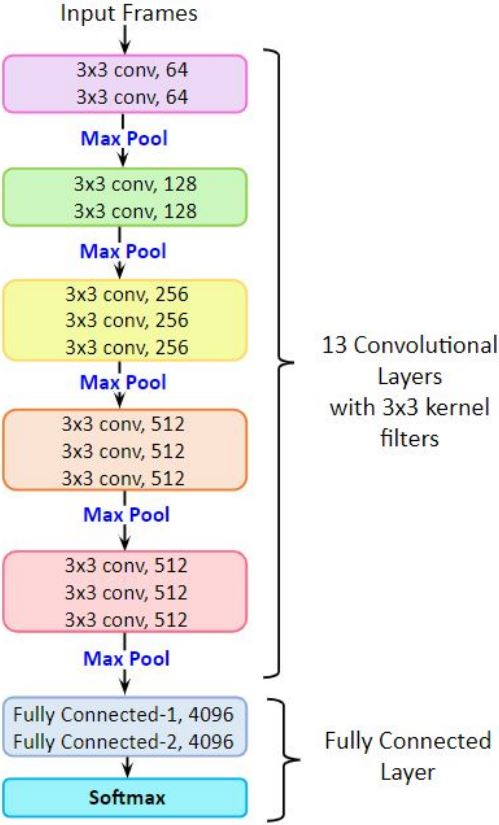
\includegraphics[width=1.25in]{vggnet}
		\caption[VGGNet]{VGGNet.}
		\label{fig:vggnet}
	\end{figure}


	\subsection{Transfer Learning Architectures - Inception Network}

	\begin{bulletedlist}
		\item While VGGNet chooses a standard 3x3 size for the convolutional kernels to simplify the architecture, an important question is, is that necessarily the best kernel size for every data set?
		\item Choosing the perfect kernel size for the convolution operation can be a difficult endeavor, due to the huge variance in the location of critical information from image to image.
		\item Choosing the right filter size to extract the information needed from an image is not straightforward, as we see from the three images of cats.
		\item So in that case, why not have filters with multiple sizes operate on the same input, and then aggregate their results somehow, like an ensemble model?  This is the core idea behind the Inception Network.
		\item The Inception Network (the winner of ILSVRC 2014), consists of certain specialized repeating blocks, each of which concatenates the outputs from multiple convolutional pathways.
		\item These blocks are also known as Inception Modules, and they represent a key point of difference between the Inception Network and other architectures (\figurename~\ref{inceptionmodule}).
		\item Hence rather than choosing between 1x1, 3x3 or 5x5 convolutional filter sizes, the Inception Module concatenates the feature maps that are produced from these filters.
		\item The importance of the Inception module can be recalled by the Hebbian Principle of Human Learning, which states that ``Neurons that fire together wire together.'' This means that when creating a new layer in a Deep Learning model, one should always pay attention to the learnings of the previous layer.
		\item Suppose a layer in our CNN has learned to focus on individual parts of the face. The next layer should then focus on the overall face in the image, and recognize it. To perform this recognition, the layers should have the appropriate filter sizes for the recognition task of that layer.  The Inception Network, unlike other architectures of the time, provides scope for this idea.
		\item What happens in the Inception Module is that by providing choices of different filter sizes, the
network itself learns to rely more on larger filter sizes (like 5x5 Convolutions) the deeper we go into the network, as those larger filter sizes are more appropriate for higher-level feature detection such as recognizing a whole face, as opposed to smaller parts like eyes or ears.
		\item The flexibility to make this choice, which was not provided by other architectures of the time, is what allowed the Inception Module, and ultimately the Inception Network, to achieve state-of-the-art performance on image prediction tasks.
		\item Prior to the Inception Network, researchers believed that increasing the depth of the network  (in terms of the number of layers) was the best way to improve performance.  With InceptionNet however, researchers realized that the width of the network (the number of feature maps concatenated together at each layer) was also important in addition to its depth, as a way to improve model performance with minimal increase in the model's computational requirements.
	\end{bulletedlist}

	\begin{figure}[tbh]
		\centering
		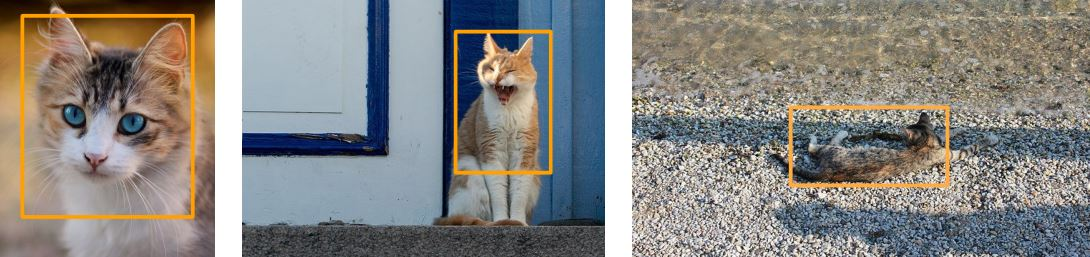
\includegraphics[width=\textwidth-1in]{inceptionnetkernalsize}
		\caption[Inception Network kernel size selection]{Inception Network kernel size selection.}
		\label{fig:inceptionnetkernalsize}
	\end{figure}

	\begin{figure}[tbh]
		\centering
		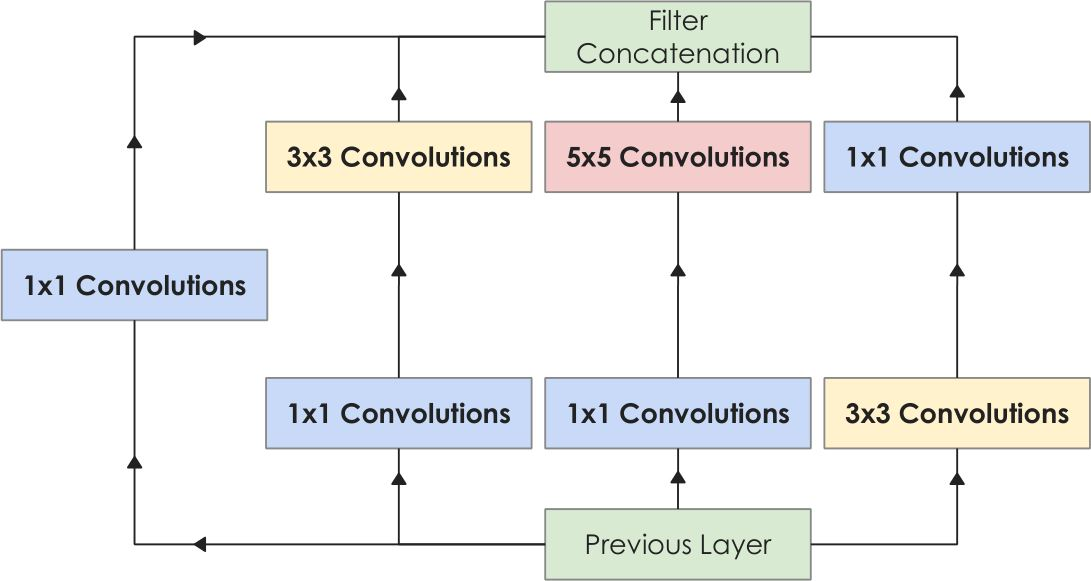
\includegraphics[width=2.5in]{inceptionmodule}
		\caption[Inception module]{Inception module.}
		\label{fig:inceptionmodule}
	\end{figure}

	\begin{figure}[tbh]
		\centering
		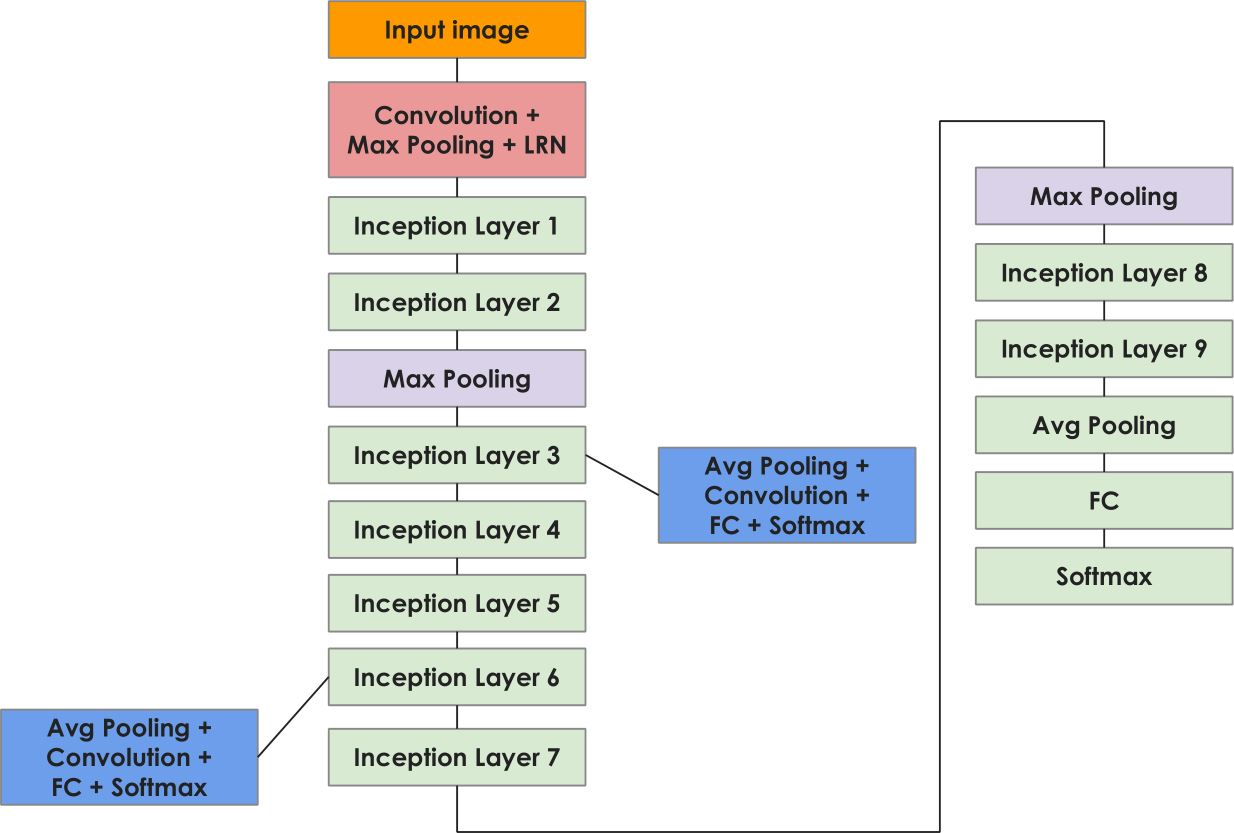
\includegraphics[width=\textwidth-2in]{inceptionnetworkexamplecnn}
		\caption[Inception Network architecture]{The Inception Network consists of multiple inception layers throughout the architecture in addition to the other, more standard, building blocks like convolution, pooling, and fully connected layers.  Another unique feature of InceptionNet is that at certain inception layers (3 and 6 in this diagram), outputs are taken at those intermediate layers as well, to create auxiliary classifiers.  The loss function combines the outputs of these auxiliary classifiers with the output of the main chain of the network, as an ensemble technique to reduce error.}
		\label{fig:inceptionnetworkexamplecnn}
	\end{figure}

	\begin{bulletedlist}
		\item As seen in the architecture diagram earlier, the Inception Network has three main structural components:
		\begin{bulletedlist}
			\item The Inception Module
			\item The [ Convolution + Max Pooling + LRN ] Module
			\item The [Average Pooling + Convolution + Fully Connected + Softmax] Module
		\end{bulletedlist}
	\end{bulletedlist}

	\subsubsection{Convolution + Max Pooling + LRN}
	\begin{bulletedlist}
		\item This is the first structural module of InceptionNet after the input image. This module has 3 Convolution layers, 2 Max Pooling layers and 2 LRN (Local Response Normalization) layers.
		\item LRN is a non-trainable layer that square-normalizes each pixel value along its entire depth across all feature maps (within the local neighborhood). The main reason for using LRN over Batch Normalization was to encourage ``lateral inhibition,'' or maintaining the contrast values of the neighborhood of an image, so that the locally maximum pixel values maintain their importance for the next layers.
	\end{bulletedlist}

	\begin{figure}[tbh]
		\centering
		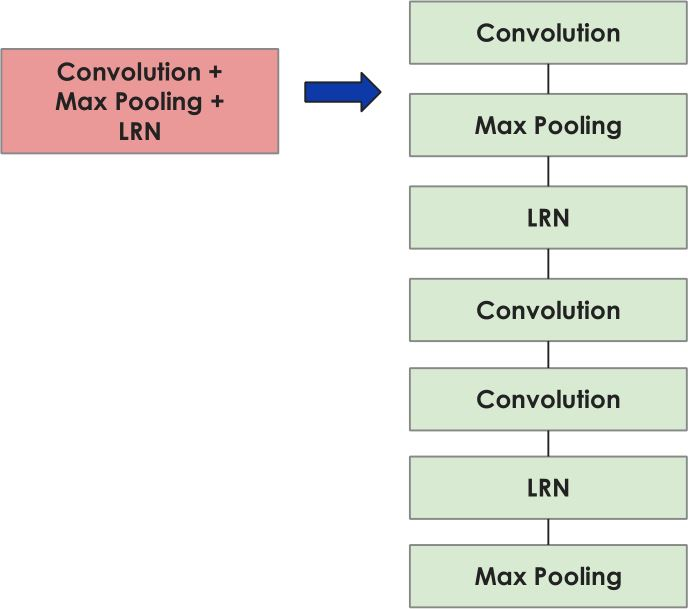
\includegraphics[height=3in]{inceptionnetworkstructuralcomponents}
		\caption[Inception structural module of convolution, max pooling, and LRN]{Inception structural module of convolution, max pooling, and LRN.}
		\label{fig:inceptionnetworkstructuralcomponents}
	\end{figure}

	\subsubsection{Average Pooling + Convolution + FC + Softmax}	
	\begin{bulletedlist}
		\item In CNNs, as the network grows deeper, the chances of the network being subject to the Vanishing Gradient problem increases.
		\item To prevent the middle of the Inception Network from dying out, two auxiliary classifiers were introduced, consisting of Average Pooling, Convolution, Fully Connected and Softmax Layers.  These auxiliary classifiers apply Softmax to the outputs of two inception modules, and compute an auxiliary loss.
		\item The total loss function of the InceptionNet equals the weighted sum of the real loss of the main chain and the auxiliary loss.
	\end{bulletedlist}

	\begin{figure}[tbh]
		\centering
		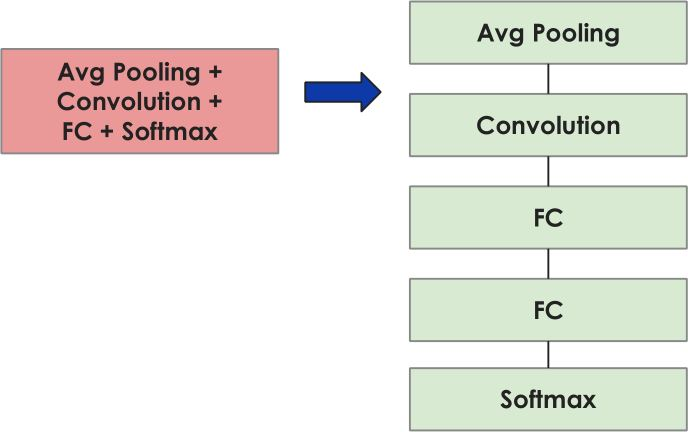
\includegraphics[height=3in]{inceptionnetworkpoolingconvolutionfcsoftmax}
		\caption[Inception structural module of average pooling, convolution, FC, and Softmax]{Inception structural module of average pooling, convolution, Fully connected, and Softmax.}
		\label{fig:inceptionnetworkpoolingconvolutionfcsoftmax}
	\end{figure}


	\subsection{Transfer Learning Architectures - Residual Networks}


	\section{Model Building Practices}
What should the order of different layers in a Convolutional Neural Network be? Where should I put my Batch Norm, Dropout, Activation, and Pooling layers?  Are there any guidelines regarding the same?

	\subsection{Dropout vs Batch Normalization}
The standard deviation issue.

There is a big problem that appears when you mix these layers, especially when Batch Normalization is right after Dropout.
Dropouts try to keep the same mean of the outputs without dropouts, but it does change the standard deviation, which will cause a huge difference in the Batch Normalization between training and validation. (During training, the Batch Normalization receives changed standard deviations, and accumulates and stores them. During validation, the dropouts are turned off, the standard deviation is not a changed one anymore, but the original. But Batch Normalization, because it's invalidation, will not use the batch statistics, but the stored statistics, which will be very different from the batch statistics).

So, the first and most important rule is: don't place a Batch Normalization after a Dropout (or a SpatialDropout).
Usually,  try to leave at least two convolutional/dense layers without any dropout before applying a batch normalization, to avoid this.

	\subsection{Dropout vs Batch Normalization}
If done in an improper order, it can result in changing the zeros to another value.

Also important, the role of the Dropout is to zero the influence of some of the weights of the next layer.  If you apply a normalization after the dropout, you will not have zeros anymore, but a certain value that will be repeated for many units.  And this value will vary from batch to batch. So, although there is noise added, you are not killing units as a pure dropout is supposed to do.

	\subsection{Dropout vs MaxPooling}
The problem of using a regular Dropout before a MaxPooling is that you will zero some pixels, and then the MaxPooling will take the maximum value, sort of ignoring part of your dropout. If your dropout happens to hit a maximum pixel, then the pooling will result in the second maximum, not in zero.
So, Dropout before MaxPooling reduces the effectiveness of the dropout.

	\subsection{Batch Normalization vs Activation}
Depending on the activation function, using a batch normalization before it can be a good advantage.
For a ReLU activation, the normalization makes the model fail-safe against a bad luck case of ``all zeros freeze a ReLU layer.''  It will also tend to guarantee that half of the units will be zero and the other half linear.

For a sigmoid or a tanh, the Batch Normalization will guarantee that the values are within a healthy range, avoiding saturation and vanishing gradients (values that are too far from zero will hit an almost flat region of these functions, causing vanishing gradients).
There are people that say there are other advantages if you do the contrary, I'm not fully aware of these advantages, I like the ones I mentioned very much.

	\subsection{Dropout vs Activation}
With ReLU, there is no difference, it can be proved that the results are exactly the same (Links to an external site.)Links to an external site.

With activations that are not centered, such as sigmoid putting a dropout before the activation will not result in zeros, but in other values.  For a sigmoid, the final results of the dropout before it would be 0.5.

If you add a tanh after a dropout, for instance, you will have the zeros, but the scaling that dropout applies to keep the same mean will be distorted by the tanh.

	\subsection{MaxPooling vs Activation}
There is nothing much here. If the activation is not very weird, the final result would be the same.

	\subsection{Conclusions}
Find the appropriate order of layers which is often useful
	\begin{bulletedlist}
	\item Group 1
		\begin{bulletedlist}
			\item Convolution
			\item Batch Norm
			\item Activation
			\item MaxPooling
			\item Dropout or SpatialDropout
		\end{bulletedlist}
	\item Group 2
		\begin{bulletedlist}
			\item Convolution
			\item ----- (there was a dropout in the last group, no Batch Norm here)
			\item Activation
			\item MaxPooling
			\item Dropout or SpatialDropout (decide to use or not)
			\item After two groups without dropout, can use Batch Norm again
		\end{bulletedlist}
	\end{bulletedlist} 